\documentclass[11pt,notes=hide,aspectratio=169,mathserif]{beamer}

% PACKAGES
\usepackage{graphics}  % Support for images/figures
\usepackage{graphicx}  % Includes the \resizebox command
\usepackage{tikz}      % For flowcharts
\usetikzlibrary{arrows.meta, positioning} % Libraries for TikZ


\usepackage{url}	   % Includes \urldef and \url commands
\usepackage{natbib}
\usepackage{bibentry}  % Includes the \nobibliography command
\usepackage{verbatim}  %Supports comments
\usepackage{booktabs} %Supports \toprule, \bottomrule, etc in tables
\usepackage{etoolbox}  %Supports toggle commands
\usepackage{datetime}
\usepackage{bm}	%Supports bold math \bm
%the LaTeX standard:
\usepackage{cmbright}
\setbeamerfont{frametitle}{family=\fontfamily{cmbr}\selectfont,size=\Large}
\fontencoding{OT1}\fontfamily{cmbr}\selectfont

% PACKAGES (that should already be included by your LyX document settings)
\usepackage{amsfonts}  % Lots of stuff, including \mathbb 
\usepackage{amsmath}   % Standard math package
\usepackage{amsthm}    % Includes the comment functions
\usepackage{subcaption}

% CUSTOM DEFINITIONS
\def\newblock{} %Get beamer to cooperate with BibTeX
\linespread{1.2}

% IDENTIFYING INFORMATION
\title[class]{ECON 326: Economics of Developing Countries \\ TA Session 7}
\author[vaidehi's class ]{Vaidehi Parameswaran (Northwestern Econ)}
\date{\monthname[\the\month] \the\year}

% THEMATIC OPTIONS
%\setbeamercovered{transparent}
\usetheme{metropolis}
\definecolor{mycolor}{RGB}{0,153,153} % define cyan colour
\setbeamercolor{frametitle}{bg=mycolor, fg=white} % Frame title color
\setbeamercolor{title separator}{fg=mycolor} 
\setbeamercolor{progress bar}{fg=mycolor} 
\beamertemplatenavigationsymbolsempty
%\setbeamertemplate{footline}[frame number]{}
\setbeamertemplate{itemize item}{\small\raisebox{1pt}{\textcolor{mycolor}{$\blacktriangleright$}}}
\setbeamertemplate{itemize subitem}{\footnotesize\raisebox{1pt}{\textcolor{mycolor}{$\triangleright$}}}
\setbeamertemplate{itemize subsubitem}{\tiny\raisebox{1pt}{\textcolor{mycolor}{$\triangleright$}}}

% BACKUP SLIDE NUMBERING
\usepackage{appendixnumberbeamer}

\begin{document}

%---------------------------------------------------------------------
\begin{frame}[plain]
\titlepage
\end{frame}
%---------------------------------------------------------------------


%---------------------------------------------------------------------
\begin{frame}{Today's Agenda}

\begin{itemize}
\item \href{https://onlinelibrary-wiley-com.turing.library.northwestern.edu/doi/epdf/10.3982/ECTA18916}{\textcolor{blue}{Beaman, Karlan, Thuysbaert \& Udry (2023)}}
\item \href{https://www.nber.org/system/files/working_papers/w16018/w16018.pdf}{\textcolor{blue}{Feigenberg, Field, \& Pande (2013)}}
\item \href{https://onlinelibrary.wiley.com/doi/abs/10.3982/ECTA5781}{\textcolor{blue}{Karlan and Zinman, (2009)}}
\end{itemize}
\end{frame}
%---------------------------------------------------------------------

\section*{\href{https://onlinelibrary-wiley-com.turing.library.northwestern.edu/doi/epdf/10.3982/ECTA18916}{\textcolor{blue}{Beaman, Karlan, Thuysbaert \& Udry (2023)}} \\[5mm] 
\textnormal{\small{Selection Into Credit Markets: Evidence from agriculture in  Mali}}}

%---------------------------------------------------------------------
\begin{frame}{Overview}

\begin{itemize}
\item Returns to investment in productive activities may be heterogenous
\item Financial markets ought to help capital flow to the highest return activities. 
\item But do they?
\item Market failures in financial and credit markets could impede efficient allocation of capital
\item This paper examines the extent to which a lending program for smallholder farmers in Mali successfully identifies and allocates credit to the farmers with higher returns to investment
\end{itemize}
\end{frame}
%---------------------------------------------------------------------

%---------------------------------------------------------------------
\begin{frame}{RCT Design I}
\begin{itemize}
    \item Two-stage RCT 
    \item Stage 1: A microcredit organisation offered group-liability loans to all women in 88 randomly selected villages in Mali 
    \item Stage 2: After decisions to take up the loan were made, a random subset of households that did not borrow in loan villages and in non-loan villages were immediately given a cash grant
    \item Key idea: identify whether those who chose not to borrow have lower average returns to a grant
\end{itemize}
\end{frame}
%---------------------------------------------------------------------

%---------------------------------------------------------------------
\begin{frame}{RCT Design II}
    \begin{figure}
            \centering
            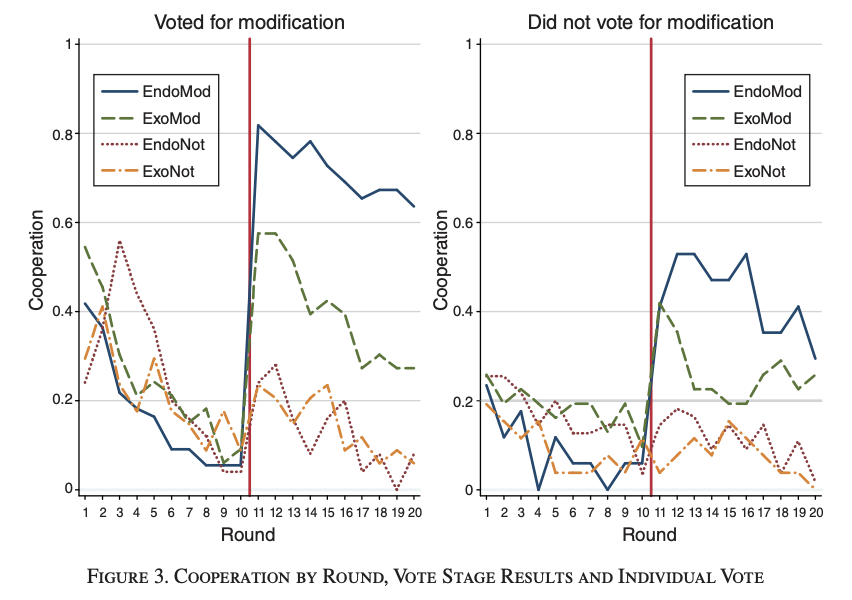
\includegraphics[width=0.8\textwidth]{inputs/fig3.png}
    \end{figure}
\end{frame}
%---------------------------------------------------------------------

%---------------------------------------------------------------------
\begin{frame}{Strategy}
\begin{itemize}
    \item We want to estimate $\beta_1$ and $\beta_2$ in
    \begin{equation*}
        Y_i = \alpha_i + \beta_1 grant_i + \beta_2 grant_i\times loan_{v(i)}+ \gamma_1 loan_{v(i)} + \epsilon_i
    \end{equation*}
    \item $Y_i$ - outcome of interest (profits)
    \item $grant_i = 1$ if household $i$ receives the cash grant
    \item $loan_{v(i)} = 1$ if household $i$ is in a village $v(i)$ that gets loans (but if so, this means $i$ got shut out of the credit market)
    \item $\beta_1$ is the effect of the cash grant in non-loan villages
    \item $\beta_2$ is the additional effect of the cash grant on households from loan villages denied loans (for them, the total effect of cash grants is $\beta_1+\beta_2$)
\end{itemize}
\end{frame}
%---------------------------------------------------------------------



%---------------------------------------------------------------------
\begin{frame}{Results I}
\begin{itemize}
    \item Within randomly selected loan villages, the ``best'' farmers seem to be the ones who get the loans
    \item They have more assets and make more profits 
\end{itemize}
\begin{figure}
    \centering
    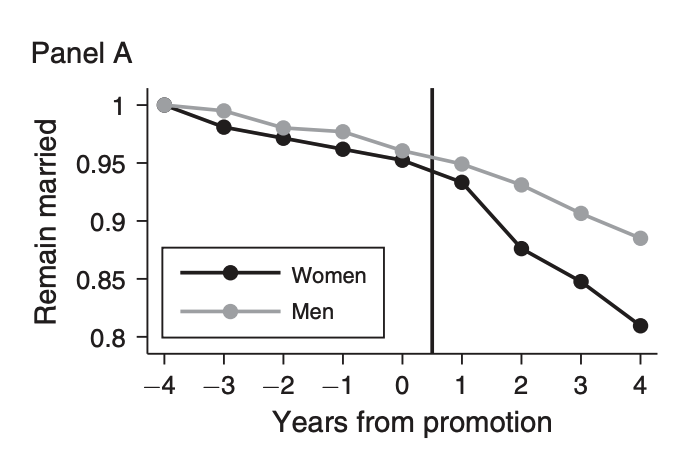
\includegraphics[width=0.6\textwidth]{inputs/fig4.png}
\end{figure}
\end{frame}
%---------------------------------------------------------------------

%---------------------------------------------------------------------
\begin{frame}{Results II}
\begin{itemize}
    \item \textbf{Main result:} Cash grant is less effective in loan villages
    \item In both loan and no-loan villages, grant recipients increase consumption
    \item But effects on recipients' economic performance, as measured by their farms' profits, are only observed in no-loan villages
    \item Suggests that those not selected into credit have lower profitability: receiving money does not raise their profits too much
\end{itemize}
\begin{figure}
    \centering
    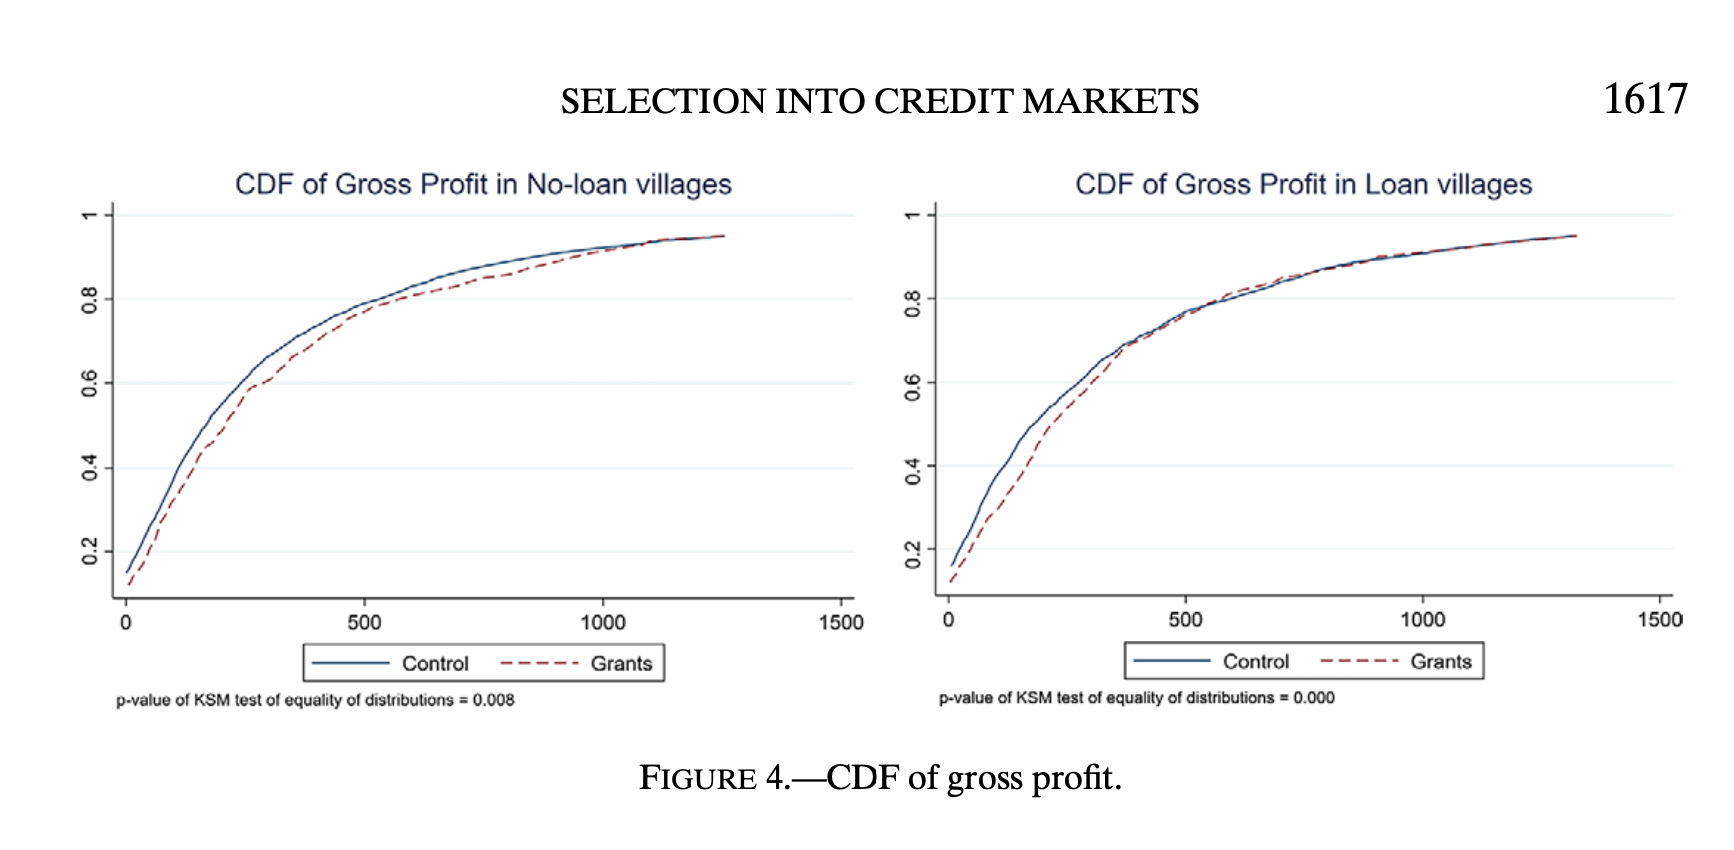
\includegraphics[width=0.4\textwidth]{inputs/fig5.png}
\end{figure}
\end{frame}
%---------------------------------------------------------------------

%---------------------------------------------------------------------
\begin{frame}{Results III}
\begin{itemize}
    \item Column 10 presents the key result: $\beta_1+\beta_2 = 0$  for profits
    \item So is it okay that these households are excluded from the credit market? 
\end{itemize}
\begin{figure}
        \centering
        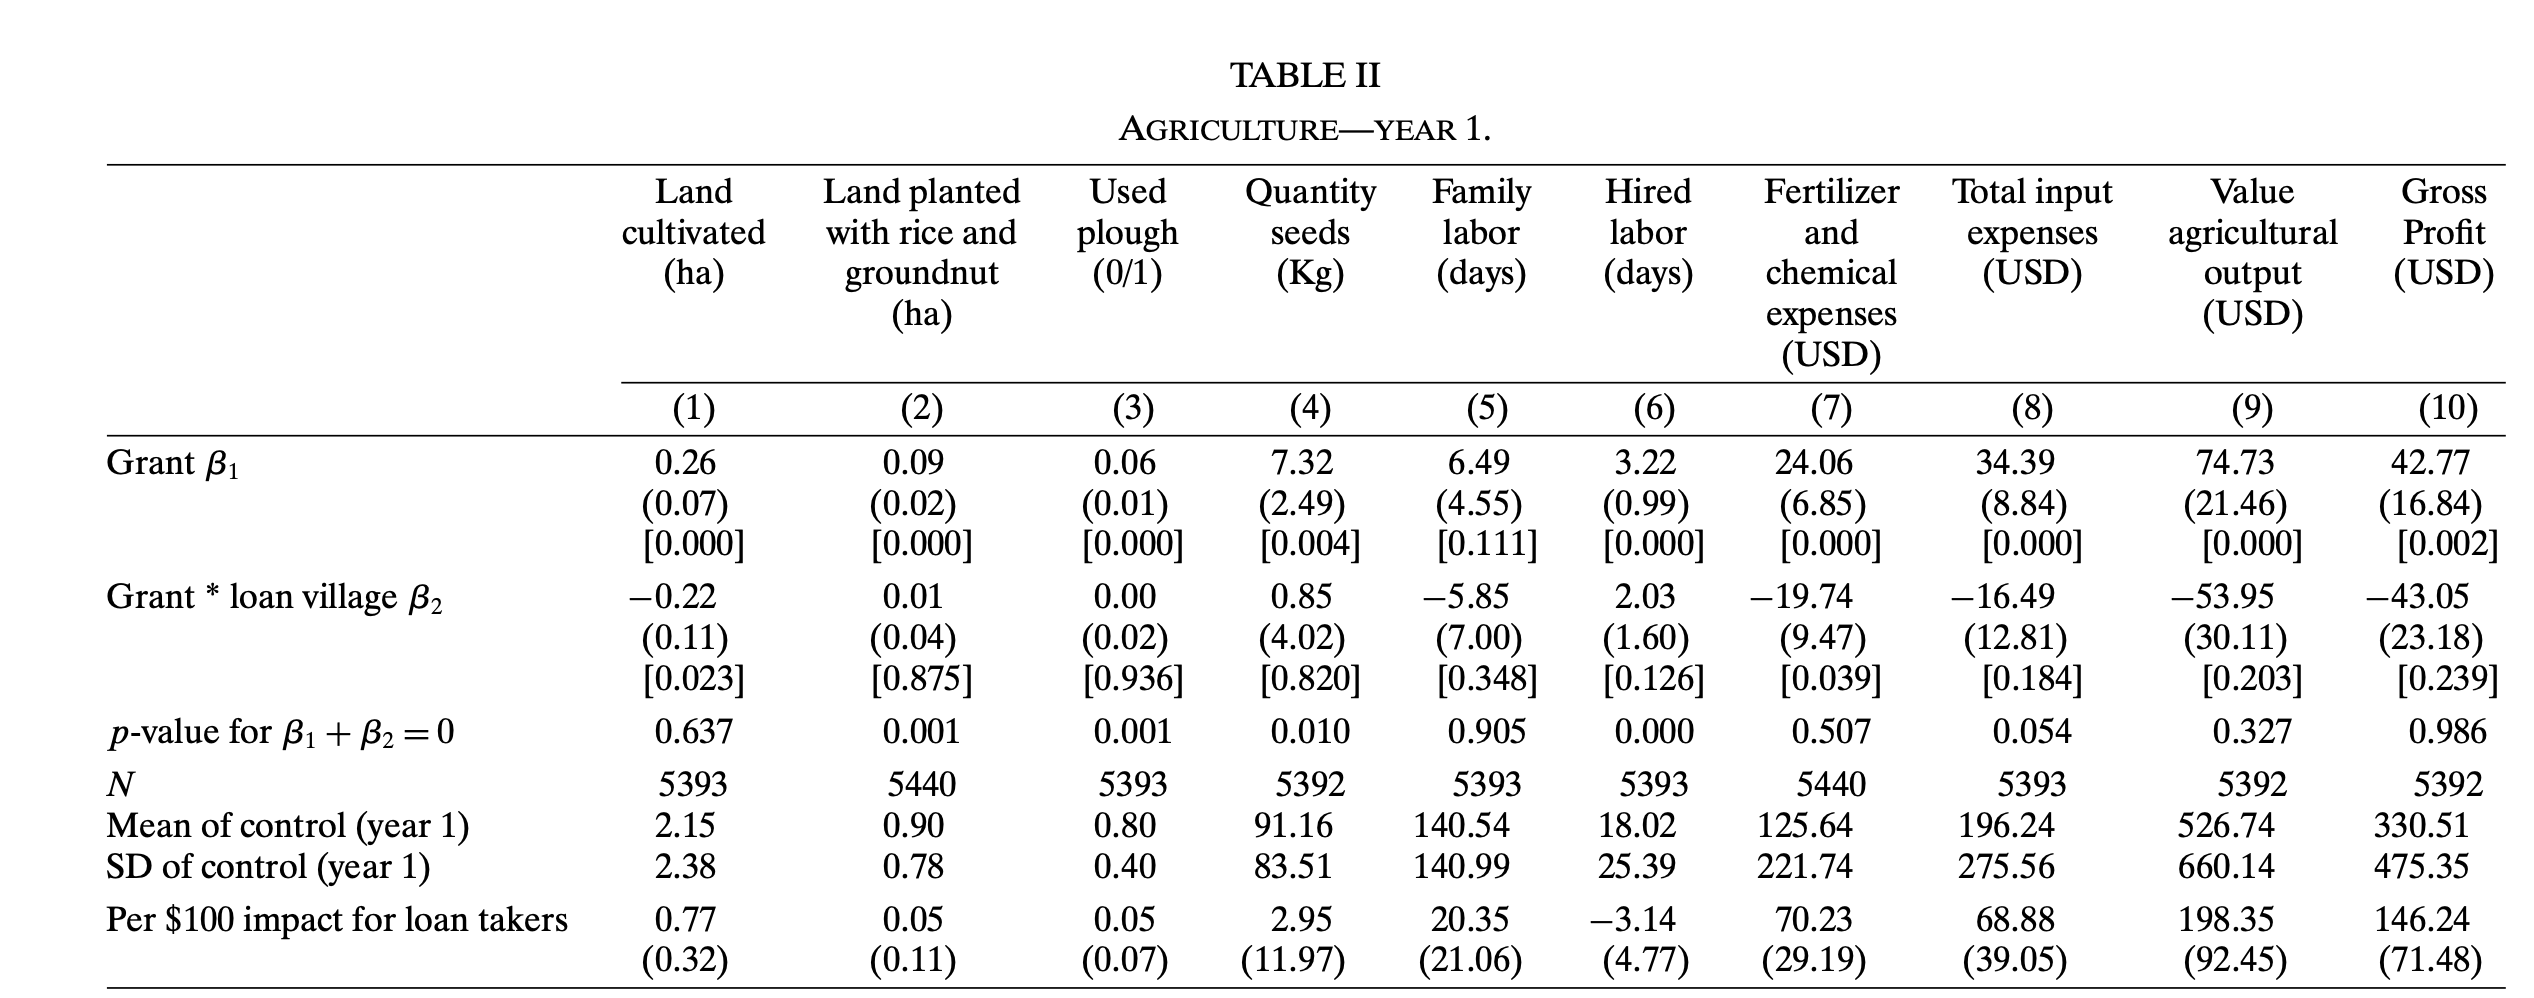
\includegraphics[width=\textwidth]{inputs/fig6.png}
\end{figure}
\end{frame}
%---------------------------------------------------------------------

\section*{\href{https://www.nber.org/system/files/working_papers/w16018/w16018.pdf}{\textcolor{blue}{Feigenberg, Field, \& Pande (2013)}} \\[5mm] 
\textnormal{\small{Building Social Capital Through Microfinance}}}


%---------------------------------------------------------------------
\begin{frame}{This paper}

\begin{itemize}
\item In developing countries, often there is a lack of formal insurance and contract enforcement mechanisms
\item Thus social capital can be particularly valuable 
\item This paper examines the role of repeated social interactions in building social capital
\end{itemize}
\end{frame}
%---------------------------------------------------------------------

%---------------------------------------------------------------------
\begin{frame}{Setting}

\begin{itemize}
\item Collaborated with a MFI in West Bengal, India 
\item A loan officer conducted a meeting to inform female residents about the loan product that was available
\item Interested women were invited to a five-day training program, after which they were assigned into groups of 10 with a team leader
\item Clients in a single group lived in close proximity to each other
\end{itemize}
\end{frame}
%---------------------------------------------------------------------

%---------------------------------------------------------------------
\begin{frame}{Experimental Design}

\begin{itemize}
\item Each group was offered an individual-liability loan of \$100 with a repayment schedule that would be assigned later 
\item Groups were randomised into weekly or monthly schedules:
\begin{itemize}
    \item Control: 38 groups who met on a monthly basis, repaid in 11 monthly installments
    \item Treatment 1: 30 groups who met on a weekly basis, repaid in 44 weekly installments
    \item Treatment 2: 32 groups who met on a weekly basis but repaid monthly 
\end{itemize}
\item Meetings:
\begin{itemize}
    \item Meetings were held in the team leader's house in the presence of as assigned loan officer
    \item Clients took an oath to repay the loan regularly and deposited payment with the loan officer 
    \item Client behaviour was observable to other team members 
    \item Compliance with meeting protocol was high in Control and Treatment 1 groups, Treatment 2 had poor compliance rates 
\end{itemize}
\end{itemize}
\end{frame}
%---------------------------------------------------------------------

%---------------------------------------------------------------------
\begin{frame}{Randomisation Check}
\begin{figure}
    \centering
    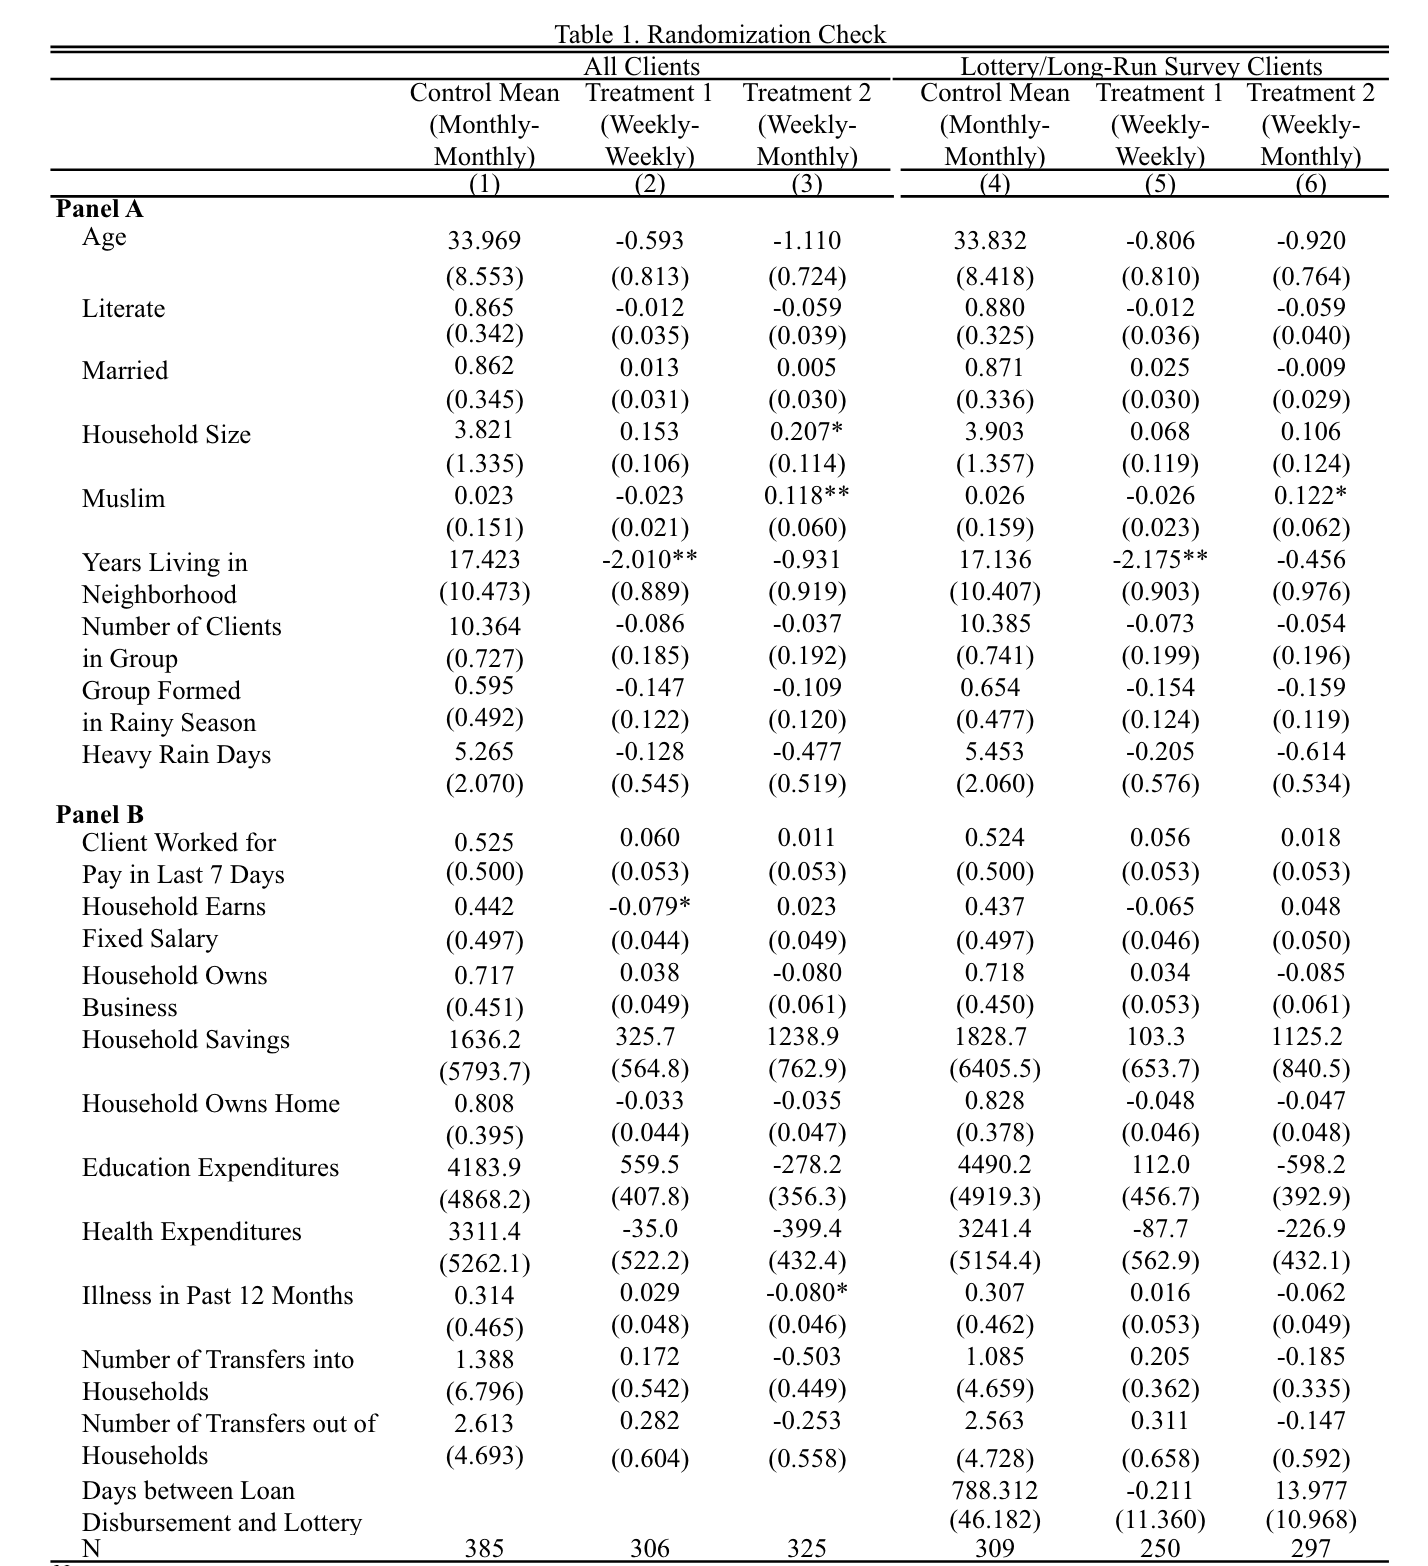
\includegraphics[width=0.5\textwidth]{inputs/Fig1.png}
\end{figure}
\end{frame}
%---------------------------------------------------------------------

%---------------------------------------------------------------------
\begin{frame}{Meeting Frequency and Social Interactions}
\begin{figure}
    \centering
    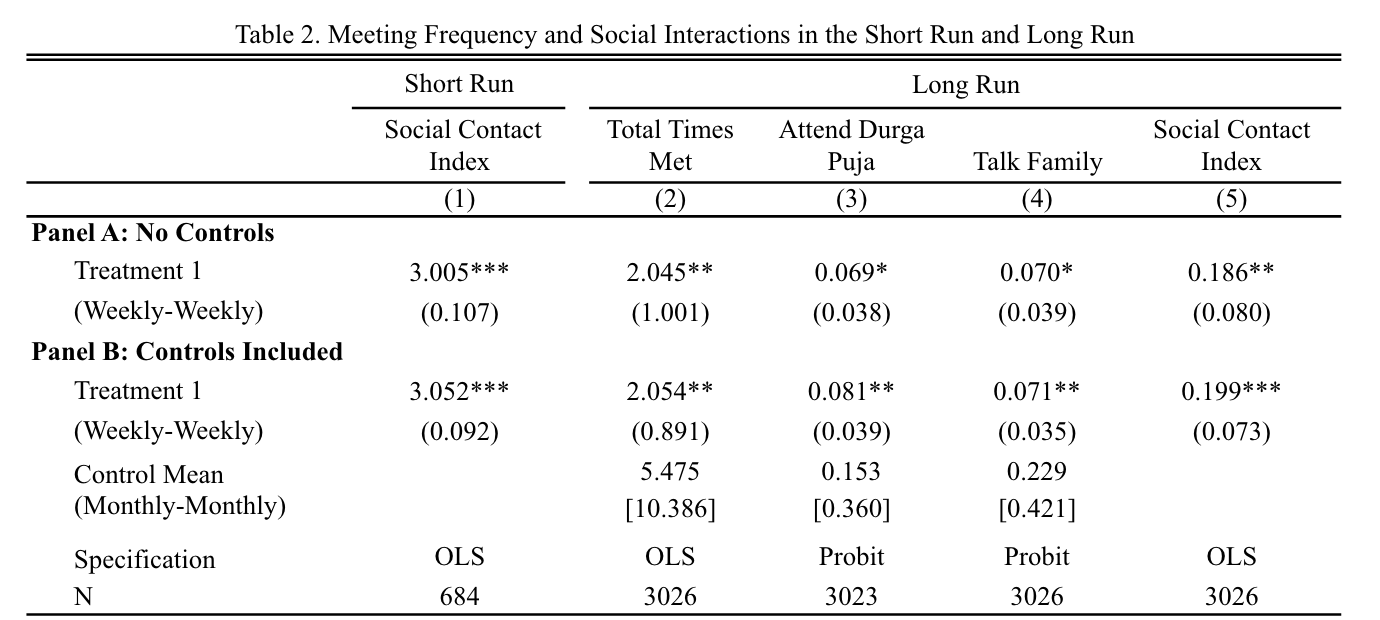
\includegraphics[width=0.6\textwidth]{inputs/Fig2.png}
\end{figure}
\begin{itemize}
    \item Use survey to ask clients about how frequently they interact with group members at the end of meetings 
    \item Switching a client from monthly to weekly meetings increases social contact with the group by over 3 sd. 
    \item These differences are persistent 
\end{itemize}
\end{frame}
%---------------------------------------------------------------------

%---------------------------------------------------------------------
\begin{frame}{Risk-sharing}
\begin{itemize}
    \item The authors examine whether increased social interaction facilitated risk-sharing arrangements 
    \item Play field-based lottery games to elicit willingness to form risk-sharing arrangements
    \item A client was chosen for the lottery and could choose to give tickets to other group members
\end{itemize}
\end{frame}
%---------------------------------------------------------------------

%---------------------------------------------------------------------
\begin{frame}{Risk-sharing II}
\begin{figure}
    \centering
    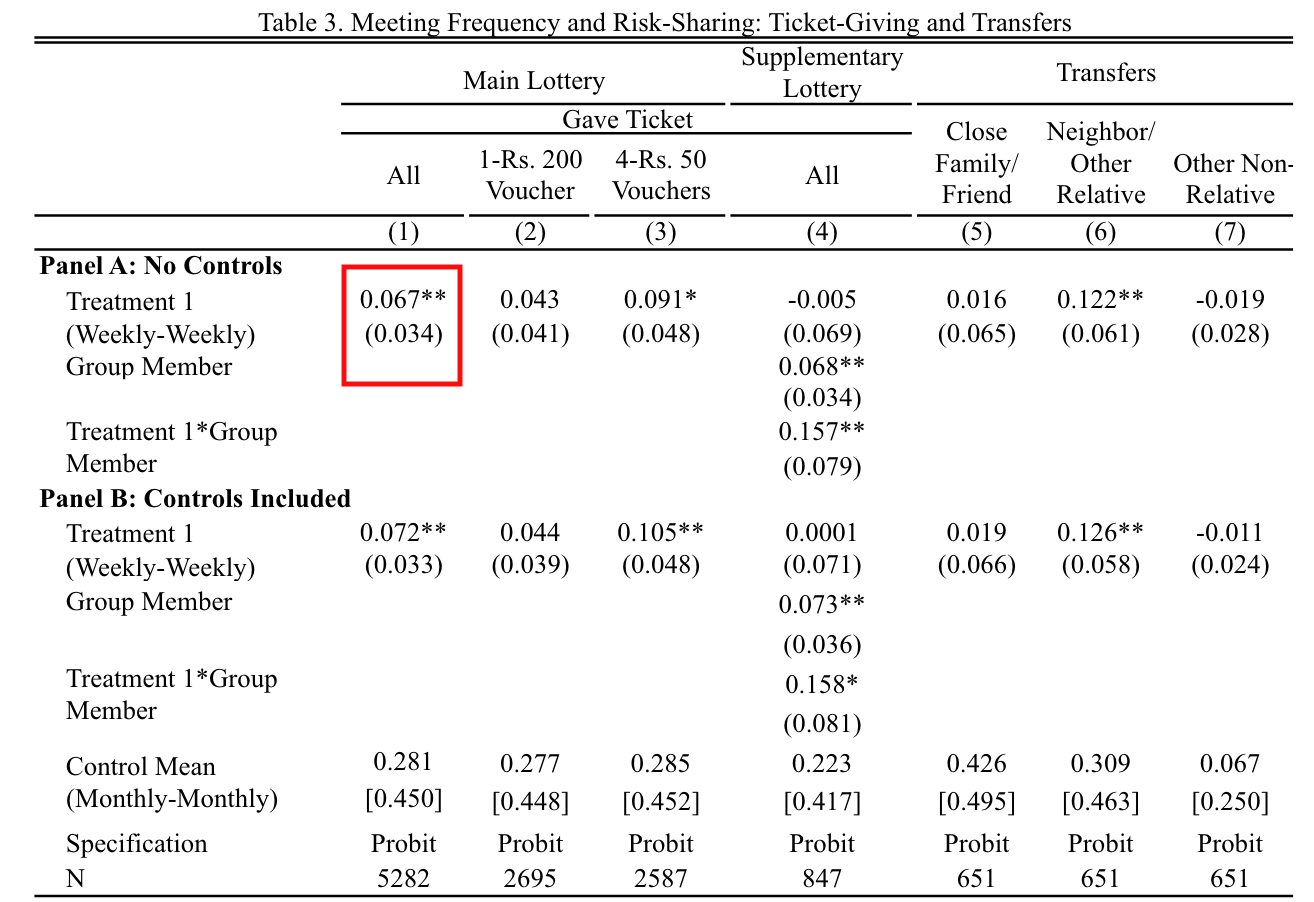
\includegraphics[width=0.5\textwidth]{inputs/table3.png}
\end{figure}
\begin{itemize}
    \item Column 1: Treatment 1 clients gave 23.8\% more tickets than the Control group 
\end{itemize}
\end{frame}
%---------------------------------------------------------------------
%---------------------------------------------------------------------
\begin{frame}{Loan Default}
\begin{figure}
    \centering
    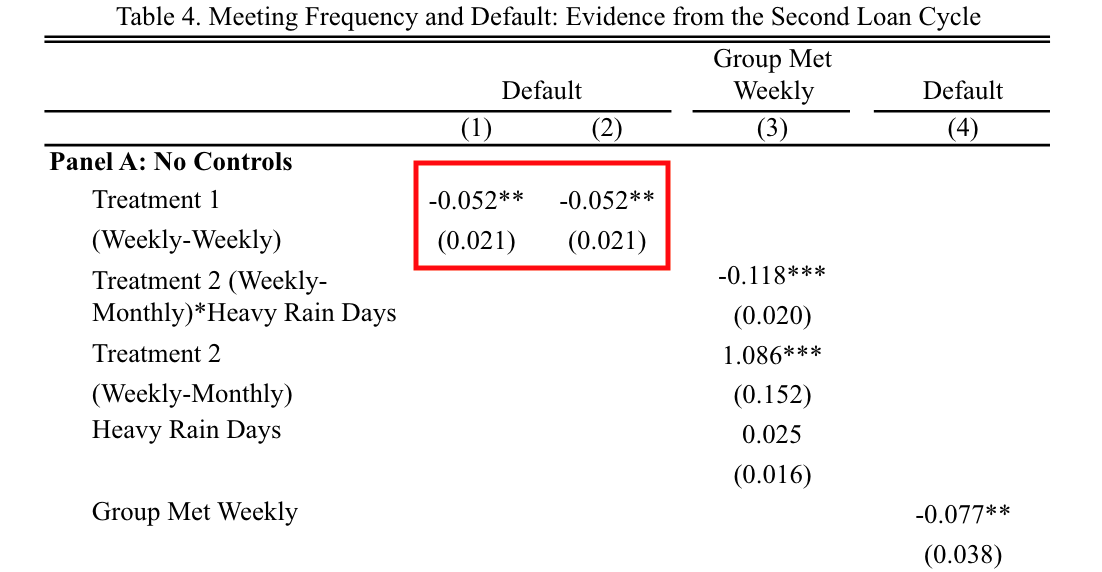
\includegraphics[width=0.6\textwidth]{inputs/table4.png}
\end{figure}
\begin{itemize}
    \item Second loan offered with same terms for both Control and Treatment 1 clients
    \item Columns (1) and (2): Treatment 1 clients nearly 3 times (5.2\%) less likely to default on second loan relative to Control 
\end{itemize}
\end{frame}
%---------------------------------------------------------------------

%---------------------------------------------------------------------
\begin{frame}{Discussion}
\begin{itemize}
    \item A program that encourages repeat interactions increases long-run social ties 
    \item Enhances social capital
    \item Improved risk-sharing in a setting where contract enforcement is weak $\rightarrow$ welfare-improving 
\end{itemize}
\end{frame}
%---------------------------------------------------------------------

\section*{\href{https://onlinelibrary.wiley.com/doi/abs/10.3982/ECTA5781}{\textcolor{blue}{Karlan and Zinman (2009)}} \\[5mm] 
\textnormal{\small{Observing Unobservables: Identifying Information Asymmetries with a Consumer Credit Field Experiment}}}

%---------------------------------------------------------------------
\begin{frame}{This paper}
\begin{itemize}
    \item Seminal work in the field of consumer finance in developing countries
    \item RCT to study the effect of interest rates on default, summarized in the figure
    \item Seeks to disentangle how interest rates affect default through (1) adverse selection, (2) moral hazard, (3) repayment burden
\end{itemize}
\begin{figure}
    \centering
    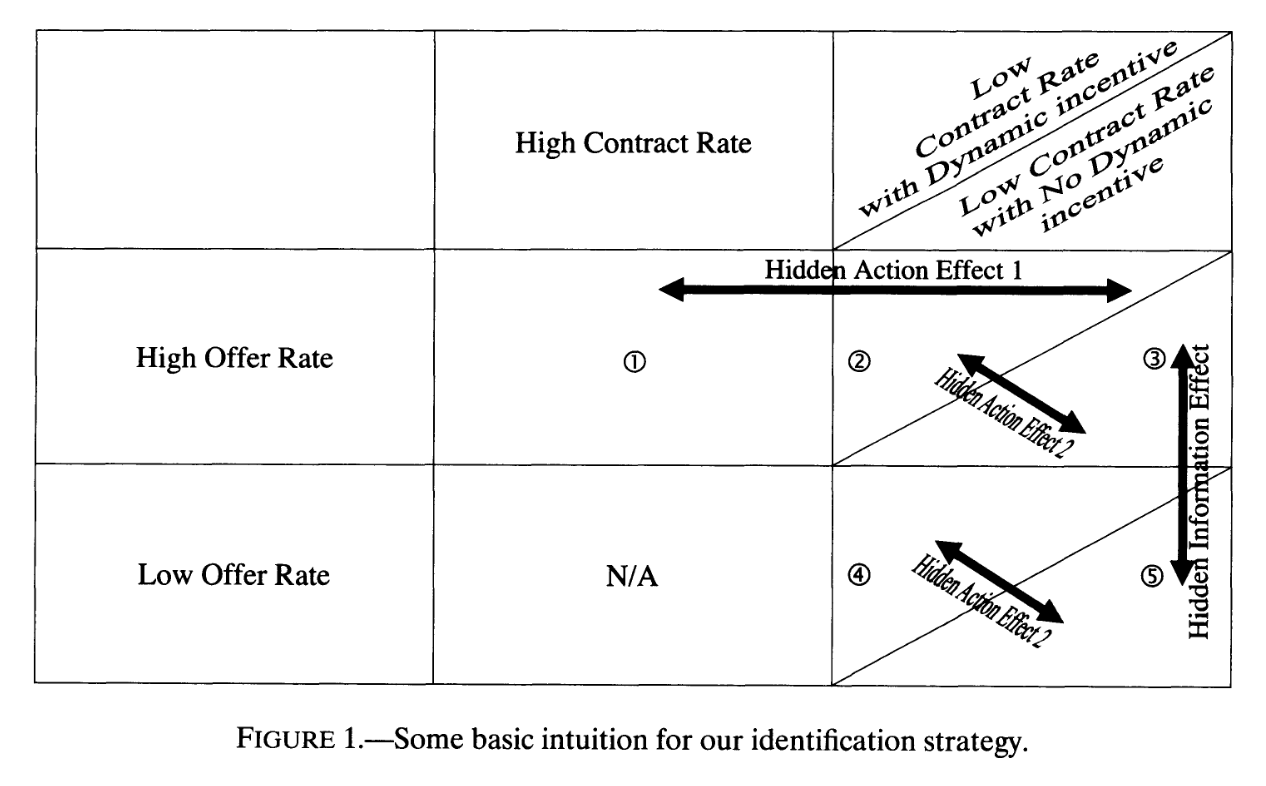
\includegraphics[width=0.5\textwidth]{inputs/main.png}
\end{figure}
\end{frame}
%---------------------------------------------------------------------

%---------------------------------------------------------------------
\begin{frame}{Adverse Selection}
\begin{figure}
    \centering
    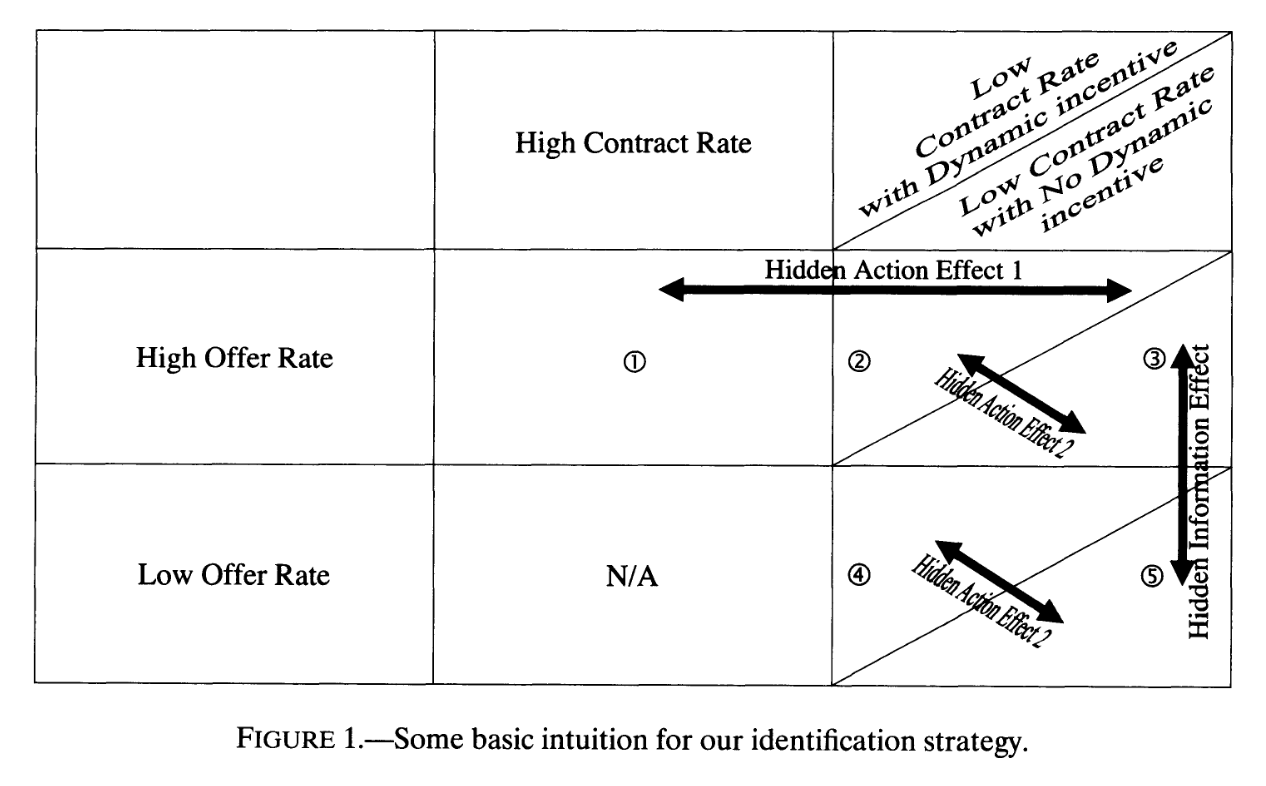
\includegraphics[width=0.35\textwidth]{inputs/main.png}
\end{figure}
\begin{itemize}
    \item The paper tests whether interest rates affect default by screening out low-quality borrowers
    \item This is done comparing 2 vs. 4 and 3 vs. 5
    \item These are pairs of groups who face the same contract rate and the same repayment incentives
    \item They only differ in the loan that was initially offered to them, which determined who accepted to participate in the study
\end{itemize}
\end{frame}
%---------------------------------------------------------------------

%---------------------------------------------------------------------
\begin{frame}{Moral Hazard}
\begin{figure}
    \centering
    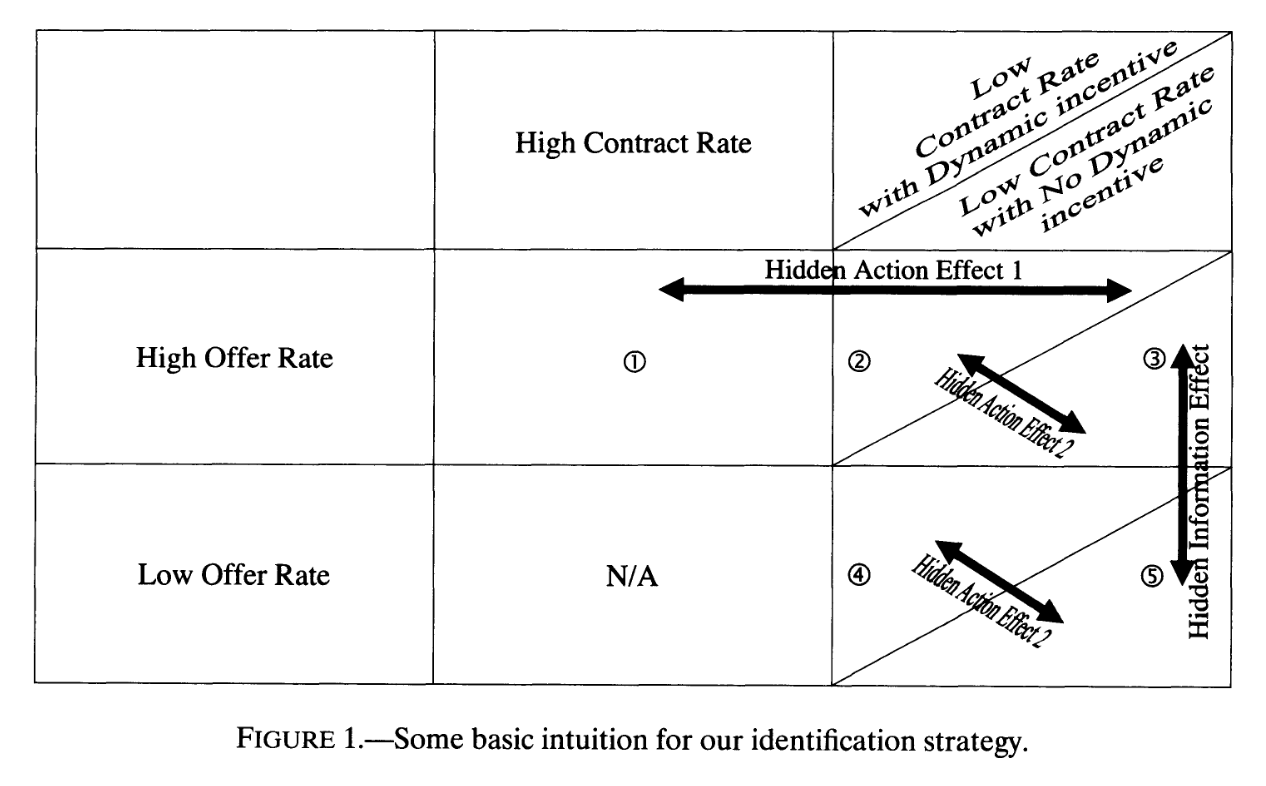
\includegraphics[width=0.35\textwidth]{inputs/main.png}
\end{figure}
\begin{itemize}
    \item The paper tests whether interest rates affect default because they are typically higher on those with bad credit histories
    \item So interest rates can be used as punishments on those who default
    \item To isolate this channel, compare 2 vs. 3 and 4 vs. 5
    \item These are pairs of groups with same offer and contract rates
    \item They differ in whether they receive a dynamic incentive: groups 2 and 4 are told that their future interest rate will depend on whether they default
\end{itemize}
\end{frame}
%---------------------------------------------------------------------

%---------------------------------------------------------------------
\begin{frame}{Repayment Burden}
\begin{figure}
    \centering
    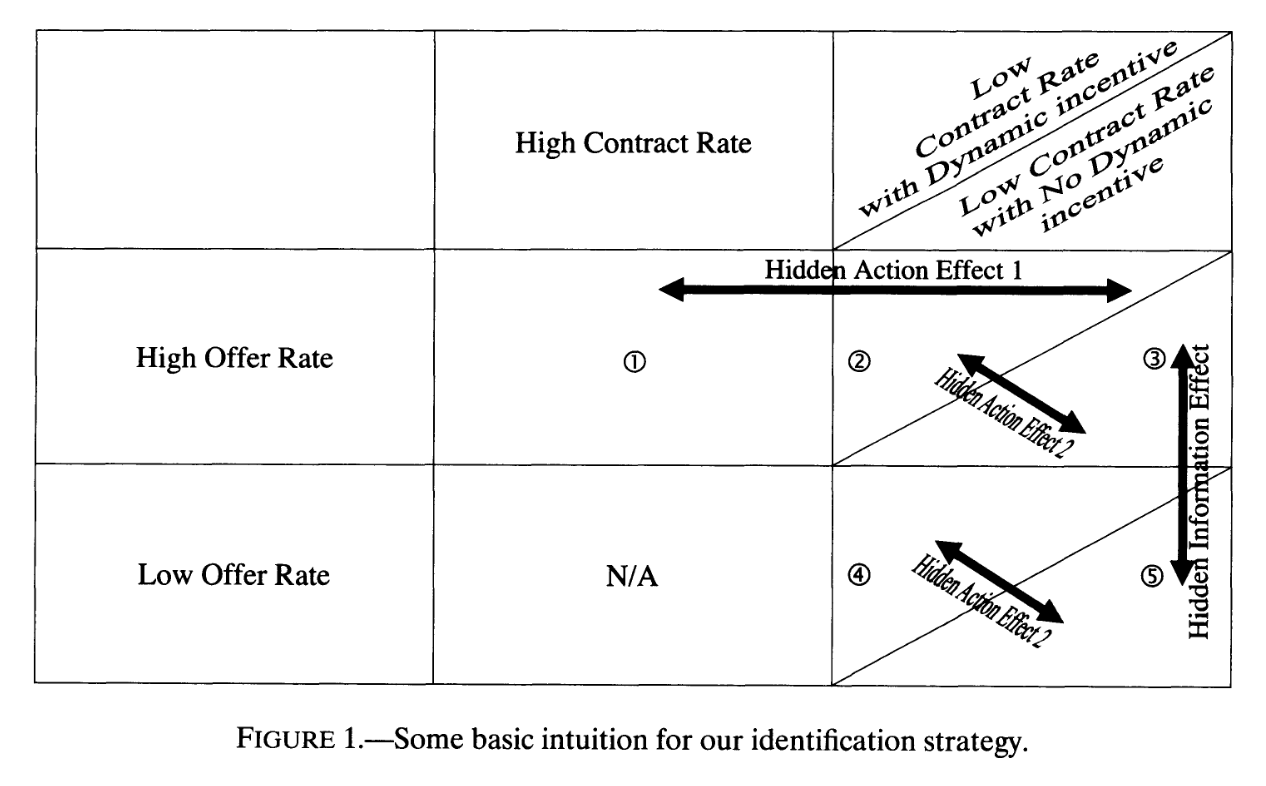
\includegraphics[width=0.35\textwidth]{inputs/main.png}
\end{figure}
\begin{itemize}
    \item The paper tests whether interest rates affect default more mechanically, by simply making the amount to be repaid higher
    \item This is done comparing 1 vs. 2 and 3
    \item A higher contract rate (on group 1) has a cost effect: the loan becomes more difficult to pay off so default will mechanically go up
    \item But the higher contract rate affects the decision to default via moral hazard too: defaulting becomes more attractive
\end{itemize}
\end{frame}
%---------------------------------------------------------------------


\end{document}
